\documentclass[12pt]{amsart}
\usepackage{amsmath,amsthm,amssymb,amsfonts,enumerate,mymath,tikz-cd,fancyhdr,multicol}
\openup 5pt
\author{Blake Farman\\University of South Carolina}
\title{Math 111\\ Exam 01\\Solutions (V2)}
\date{September 28, 2017}
\pdfpagewidth 8.5in
\pdfpageheight 11in
\usepackage[margin=1in]{geometry}

\renewcommand{\qedsymbol}{}

\begin{document}
\maketitle

\theoremstyle{definition}
\newtheorem{thm}{}
\newtheorem{defn}{Definition}
\newtheorem*{rmk}{Remark}

\section{Definitions}
\begin{thm}[3 Points]\label{ex1}
  Fill in the blanks with the correct factorizations.
  \begin{enumerate}[(a)]
  \item
    $\displaystyle{A^2 - B^2 = (A - B)(A + B)}.$
    \vspace{.3in}
  \item
    $\displaystyle{A^2 + 2AB + B^2 = (A + B)^2}.$
    \vspace{.3in}
  \item
    $\displaystyle{A^2 - 2AB + B^2 = (A - B)^2}.$
    \vspace{.3in}
  \end{enumerate}
\end{thm}
\vspace{.5in}
\begin{thm}[6 Points]\label{ex2}
    Let $a, b$ be non-zero real numbers and $m, n$ integers.
  Fill in the blanks
  \vspace{.25in}
  \begin{multicols}{2}
    \begin{enumerate}
    \item
      $\displaystyle{a^0 = 1}$
      \vspace{.4in}
    \item
      $\displaystyle{a^{-n} = \frac{1}{a^n}}$
      \vspace{.3in}
    \item
      $\displaystyle{a^m \cdot a^n = a^{m+n}}$
    \item
      $\displaystyle{\frac{a^m}{a^n}= a^{m-n}}$
      \vspace{.25in}
    \item
      $\displaystyle{\left(a \cdot b\right)^n = a^n b^n}$
      \vspace{.25in}
    \item
      $\displaystyle{\left(\frac{a}{b}\right)^n = \frac{a^n}{b^n}}$
    \end{enumerate}
  \end{multicols}
\end{thm}
\newpage
\begin{thm}[2 Points]\label{ex3}
  Given a Quadratic Equation, $ax^2 + bx + c = 0$, the solutions are given by the Quadratic Formula.  State the Quadratic Formula.

  $$x = \frac{-b \pm \sqrt{b^2 - 4ac}}{2a}.$$
\end{thm}

\begin{thm}[3 Points]\label{ex4}
  Fill in the blanks:\\
  \begin{center}
    To make $x^2 + bx$ a perfect square, add $\left(\frac{b}{2}\right)^2$.
    This gives the perfect square
    \vspace{.5in}
    $$x^2 + bx + \left(\frac{b}{2}\right)^2 = \left(x + \frac{b}{2}\right)^2.$$
  \end{center}
\end{thm}
\vspace{.5in}
\begin{thm}[3 Points]\label{ex5}
Fill in the blanks:\\
  \begin{center}
    An equation in variables $x$ and $y$ defines the variable $y$ as function of the variable $x$ if\\
    \vspace{.2in}
    each value of $x$ corresponds to exactly one value of $y$.
  \end{center}
\end{thm}
\vspace{.5in}
\begin{thm}[3 Points]\label{ex6}
    Let $f(x)$ be a function of the variable $x$, and assume that $a \leq b$ are real numbers.
  State the formula for the net change between the inputs $x = a$ and $x = b$.\\
  
  \vspace{.5in}
  The net change is given by the formula
  $$f(b) - f(a).$$
\end{thm}

\newpage
\section{Problems}
\begin{thm}[16 Points]\label{ex7}
  Consider the equation
  $$y^2 + 2x = 6.$$
  \begin{enumerate}[(a)]
    \item
      Does this equation define $y$ as function of $x$?  
      \emph{Briefly} justify why or why not.
      If it does, then give the value of $y$ when $x = 2$.
      \begin{proof}[Solution]
        This equation does \emph{not} define $y$ as a function of $x$.
      When $x = 2$ we have the equation
      $$6 = y^2 + 2(2) = y^2 + 4.$$
      Subtracting 4 from both sides yields
      $$y^2 = 6 - 4 = 2$$
      so there are two choices for value of $y$: either $\sqrt{2}$ or $-\sqrt{2}$.
      \end{proof}
    \item
      Does this equation define $x$ as function of $y$?  \emph{Briefly} justify why or why not.
      If it does, then give the value of $x$ when $y = 2$.
      \begin{proof}[Solution]
        This equation does define $x$ as a function of $y$.
        Subtracting $y^2$ from both sides we obtain
        $$2x = 6 - y^2.$$
        Dividing both sides by $2$ we obtain
        $$x = \frac{6 - y^2}{2}$$
        and this is clearly a function.
        When $y = 2$,
        $$x = \frac{6 - 2^2}{2} = \frac{6 - 4}{2} = \frac{2}{2} = 1.$$
    \end{proof}
  \end{enumerate}
\end{thm}

\begin{thm}[16 Points]\label{ex8}
  Let $f(x) = x^2 + x + 1$.  Compute the net change between $x = 1$ and $x = 4$.
  \begin{proof}[Solution]
    The net change is given by
    $$f(4) + f(1) = (4^2 + 4 + 1) - (1^2 + 1 + 1) = 21 - 3 = 18.$$
  \end{proof}
\end{thm}

\newpage

\begin{thm}[16 Points]\label{ex9}
  Add the following rational expressions and simplify the result,
  $$\frac{6}{9 - x^2} + \frac{-1}{3 + x}.$$

  \begin{proof}[Solution]
    First, we must factor the denominators to determine the least common multiple.
    The denominator $3 + x$ cannot be factored any further, but
    $$9 - x^2 = (3 - x)(3 + x).$$
    This tells us common denominator is $9 - x^2$, so
    \begin{eqnarray*}
      \frac{6}{9 - x^2} + \frac{-1}{3 + x} &=& \frac{6}{9 - x^2} + \left(\frac{3 - x}{3 - x}\right)\frac{-1}{3 + x}.\\
      &=& \frac{6}{9 - x^2} + \frac{-3 + x}{9 - x^2}\\
      &=& \frac{6 - 3 + x}{9 - x^2}\\
      &=& \frac{3 + x}{(3 + x)(3 - x)}\\
      &=& \frac{1}{3 - x}.
    \end{eqnarray*}
  \end{proof}
\end{thm}

\begin{thm}[16 Points]\label{ex10}
  Solve the equation
  $$2x^2 - 2x - 24 = 0$$
  for $x$.
  \begin{proof}[Solution]
    We first observe that we can factor a 2 out of the left-hand side to get
    $$2(x^2 - x - 12) = 0.$$
    By the Zero Factor Property, this says that either $2 = 0$ or $x^2 - x - 12 = 0$; since the first equation is nonsense, it is equivalent to solve the equation
    $$x^2 - x - 12 = 0.$$
    One either observes that
    $$x^2 - x - 12 = (x - 4)(x + 3) = 0$$
    implies by the Zero Factor Property that the solutions are $x = 4$ and $x = -3$, or uses the Quadratic Formula
    \begin{eqnarray*}
      x &=& \frac{-(-1) \pm \sqrt{(-1)^2 - 4(1)(-12)}}{2(1)}\\
      &=& \frac{1 \pm \sqrt{1 + 48}}{2}\\
      &=& \frac{1 \pm \sqrt{49}}{2}\\
      &=& \frac{1 \pm 7}{2}\\
    \end{eqnarray*}
    to see that the the solutions are given by
    $$x = \frac{1 + 7}{2} = \frac{8}{2} = 4$$
    and
    $$x = \frac{1 - 7}{2} = \frac{-6}{2} = -3.$$
  \end{proof}
\end{thm}

\begin{thm}[16 Points]\label{ex11}
  Find the domain of the function
  $$f(x) = \sqrt{x^2 - 2x - 3}.$$
  Express the solution using interval notation and graph the domain on the number line.

  \begin{proof}[Solution]
    We first observe that for $f$ to be well-defined at $x$, the value of $x^2 - 2x - 3$ must be non-negative.
    Hence finding the domain of $f$ is equivalent to solving the quadratic inequality
    $$0 \leq x^2 - 2x - 3.$$

    We first solve the equation
    $$x^2 - 2x - 3 = (x - 3)(x + 1) = 0$$
    to see that equality is obtained whenever $x = -1$ or $x = 3$.
    To find the rest of the solutions to the inequality, we must check one number from each of the intervals $(-\infty, -1)$, $(-1,3)$, and $(3,\infty)$.
    We check the signs at $x = -2$, $x = 0$, and $x = 4$.

When $x = -2$, we have
    $$(-2)^2 - 2(-2) - 3 = (-2 - 3)(-2 + 1) = (-5)(-1) = 5 > 0.$$
This tells us that $x^2 - 2x - 3$ is positive on the interval $(-\infty, -11)$

When $x = 0$, we have
$$0^2 - 2(0) - 3 = -3 < 0.$$
This tells us that $x^2 - 2x - 3$ is negative on the interval $(-1,3)$.

    When $x = 4$, we have
    $$(4)^2 - 2(4) - 3 = (4 - 3)(4 + 1) = (1)(5) = 5 > 0.$$
    This tells us that $x^2 - 2x - 3$ is positive on the interval $(3, \infty)$.
    
Combining this information, we have found that the inequality
$$0 \leq x^2 - 2x - 3$$
    is true on the intervals $(-\infty, -1)$ and $(3,\infty)$.
    In interval notation, the solutions are therefore
    $$(-\infty, -1) \cup (3,\infty).$$
    We can represent this union of intervals on the number line as
    \vspace{.5in}
    \begin{center}
      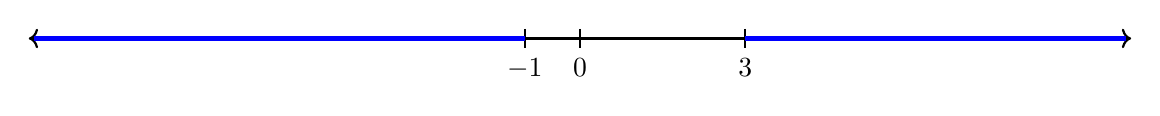
\begin{tikzpicture}[scale=7]
        \draw[<->, thick] (-1,0) -- (1,0);
        \foreach \x/\xtext in {-0.1/$-1$,0/0,0.3/$3$}
        \draw[thick] (\x,0.5pt) -- (\x,-0.5pt) node[below] {\xtext};
        \draw[{-]}, ultra thick, blue] (-.99,0) -- (-.1,0);
          \draw[[-, ultra thick, blue] (.3,0) -- (.99,0);
      \end{tikzpicture}
    \end{center}
  \end{proof}
\end{thm}

\begin{thm}[Bonus - 10 Points]\label{bonus}
  Consider the function
  $$p(x) = x^2 + 5x + 6.$$
  \begin{enumerate}[(a)]
  \item
    Find two numbers, $a < b$, for which the net change of $p$ from $a$ to $b$ is 6.
    \begin{proof}[Solution]
      This question simply asks that we find two values $a < b$ such that
      $$f(b) - f(a) = 6.$$
      The easiest possible solution would be to find $a$ and $b$ such that $f(b) = 6$ and $f(a) = 0$.
      This is equivalent to solving the two equations
      $$x^2 + 5x + 6 = 6\ \text{and}\ x^2 + 5x + 6 = 0$$
      for $x$ and identifying a solution to the first equation which is larger than some solution to the second equation.

      To solve the first, we subtract 6 from both sides to obtain
      $$x^2 + 5x = x(x + 5) = 0$$
      and note that this means either $x = 0$ or $x = -5$.
      For the second, we can factor
      $$x^2 + 5x + 6 = (x + 3)(x + 2) = 0$$
      to see that either $x = -3$ or $x = -2$.

      By some luck, we find two possible solutions.
      If we take $a = -2$, then we can take $b = 0$ since
      $$f(0) - f(-2) = 6 - 0 = 6.$$
      Similarly, if we take $a = -3$, then we can also take $b = 0$ since
      $$f(0) - f(-3) = 6 - 0 = 0.$$
    \end{proof}
  \item
    Find two numbers, $c < d$, for which the net change of $p$ from $c$ to $d$ is -6.
    \newline
        [Hint: Your method from part (a) should also give you these values.]

        \begin{proof}[Solution]
          Again, we observe that the easiest thing we could do is find two numbers, $c < d$, such that $f(d) = 0$ and $f(c) = 6$ so that the net change is
          $$f(d) - f(c) = 0 - 6 = -6.$$
          Using our work from part (a), we can take $c = -5$ and either $d = -2$ or $d = -3$ since
          $$f(-2) - f(-5) = 0 - 6 = -6$$
          and
          $$f(-3) - f(-5) = 0 - 6 = -6.$$
        \end{proof}
  \end{enumerate}
\end{thm}

\begin{rmk}
  There may well be many more solutions.
  These are just the easiest such solutions.
\end{rmk}
\end{document}
